\begin{tikzpicture}[remember picture,overlay, shift={(current page.north west)}, >=latex]
	\definecolor{coverblue}{HTML}{ffd33c}
	%\definecolor{coverpink}{HTML}{0f97e8}
  \definecolor{coverpink}{HTML}{003d5c}
	\definecolor{coveraccentpink}{HTML}{ffd33c}
	\definecolor{coverorange}{HTML}{ffffff}
	%\definecolor{covershade}{HTML}{0f004d}
  \definecolor{covershade}{HTML}{00214a}
\definecolor{c1f958c}{RGB}{31,149,140}
\definecolor{c3ab3cd}{RGB}{58,179,205}
\definecolor{cede632}{RGB}{237,230,50}
\definecolor{c2d70b3}{RGB}{45,112,179}



	\newcommand{\LINEARALGEBRAoutline}{(0.9395, 22.9548) -- (1.2851, 22.9548).. controls (1.5101, 22.9548) and (1.6447, 22.9769) .. (1.7652, 23.0372).. controls (1.9943, 23.1497) and (2.1289, 23.3948) .. (2.1289, 23.6941).. controls (2.1289, 23.9774) and (2.0123, 24.2084) .. (1.8054, 24.333).. controls (1.6889, 24.4033) and (1.5121, 24.4395) .. (1.2791, 24.4395) -- (0.9395, 24.4395) -- cycle(1.2148, 23.218) -- (1.2148, 24.1763) -- (1.269, 24.1763).. controls (1.4458, 24.1763) and (1.5382, 24.1602) .. (1.6246, 24.116).. controls (1.7652, 24.0437) and (1.8516, 23.885) .. (1.8516, 23.6941).. controls (1.8516, 23.5153) and (1.7693, 23.3566) .. (1.6367, 23.2843).. controls (1.5543, 23.2401) and (1.4398, 23.218) .. (1.275, 23.218) -- cycle(2.3177, 22.9548) -- (2.5849, 22.9548) -- (2.5849, 24.0678) -- (2.3177, 24.0678) -- cycle(2.3177, 24.1884) -- (2.5849, 24.1884) -- (2.5849, 24.4395) -- (2.3177, 24.4395) -- cycle(3.0831, 24.0477).. controls (3.0852, 24.1502) and (3.1193, 24.1823) .. (3.2258, 24.1823) -- (3.2499, 24.1823) -- (3.2499, 24.4355).. controls (3.2177, 24.4395) and (3.2037, 24.4395) .. (3.1836, 24.4395).. controls (3.0671, 24.4395) and (2.9727, 24.3973) .. (2.9043, 24.3149).. controls (2.8501, 24.2506) and (2.83, 24.1863) .. (2.8159, 24.0477) -- (2.7195, 24.0477) -- (2.7195, 23.8247) -- (2.8159, 23.8247) -- (2.8159, 22.9548) -- (3.0831, 22.9548) -- (3.0831, 23.8247) -- (3.3162, 23.8247) -- (3.3162, 22.9548) -- (3.5834, 22.9548) -- (3.5834, 23.8247) -- (3.7341, 23.8247) -- (3.7341, 24.0477) -- (3.5834, 24.0477).. controls (3.5854, 24.1502) and (3.6196, 24.1823) .. (3.726, 24.1823) -- (3.7501, 24.1823) -- (3.7501, 24.4355).. controls (3.718, 24.4395) and (3.7039, 24.4395) .. (3.6838, 24.4395).. controls (3.5673, 24.4395) and (3.4729, 24.3973) .. (3.4026, 24.3149).. controls (3.3503, 24.2506) and (3.3303, 24.1884) .. (3.3162, 24.0477) -- cycle(4.9797, 23.3928).. controls (4.9877, 23.433) and (4.9897, 23.4571) .. (4.9897, 23.4973).. controls (4.9897, 23.8408) and (4.7466, 24.0939) .. (4.4151, 24.0939).. controls (4.0877, 24.0939) and (3.8285, 23.8348) .. (3.8285, 23.5073).. controls (3.8285, 23.1818) and (4.0917, 22.9287) .. (4.4312, 22.9287).. controls (4.614, 22.9287) and (4.7567, 22.995) .. (4.8732, 23.1296).. controls (4.9154, 23.1818) and (4.9435, 23.228) .. (4.9616, 23.2843) -- (4.6703, 23.2843).. controls (4.602, 23.2039) and (4.5357, 23.1738) .. (4.4252, 23.1738).. controls (4.2665, 23.1738) and (4.1499, 23.2582) .. (4.1178, 23.3928) -- cycle(4.1097, 23.6278).. controls (4.1519, 23.7725) and (4.2604, 23.8488) .. (4.4191, 23.8488).. controls (4.5839, 23.8488) and (4.6924, 23.7705) .. (4.7265, 23.6278) -- cycle(5.1625, 22.9548) -- (5.4297, 22.9548) -- (5.4297, 23.5736).. controls (5.4236, 23.7383) and (5.508, 23.8308) .. (5.6687, 23.8368) -- (5.6687, 24.0939) -- (5.6486, 24.0939).. controls (5.5341, 24.0939) and (5.4779, 24.0618) .. (5.4076, 23.9593) -- (5.4076, 24.0678) -- (5.1625, 24.0678) -- cycle(6.8701, 23.3928).. controls (6.8782, 23.433) and (6.8802, 23.4571) .. (6.8802, 23.4973).. controls (6.8802, 23.8408) and (6.6371, 24.0939) .. (6.3056, 24.0939).. controls (5.9781, 24.0939) and (5.719, 23.8348) .. (5.719, 23.5073).. controls (5.719, 23.1818) and (5.9821, 22.9287) .. (6.3217, 22.9287).. controls (6.5045, 22.9287) and (6.6471, 22.995) .. (6.7637, 23.1296).. controls (6.8058, 23.1818) and (6.834, 23.228) .. (6.852, 23.2843) -- (6.5607, 23.2843).. controls (6.4924, 23.2039) and (6.4261, 23.1738) .. (6.3156, 23.1738).. controls (6.1569, 23.1738) and (6.0404, 23.2582) .. (6.0083, 23.3928) -- cycle(6.0002, 23.6278).. controls (6.0424, 23.7725) and (6.1509, 23.8488) .. (6.3096, 23.8488).. controls (6.4744, 23.8488) and (6.5828, 23.7705) .. (6.617, 23.6278) -- cycle(7.0529, 22.9548) -- (7.3201, 22.9548) -- (7.3201, 23.4792).. controls (7.3201, 23.6278) and (7.3302, 23.6921) .. (7.3643, 23.7464).. controls (7.4065, 23.8127) and (7.4748, 23.8488) .. (7.5612, 23.8488).. controls (7.6315, 23.8488) and (7.6858, 23.8247) .. (7.7219, 23.7785).. controls (7.7581, 23.7303) and (7.7742, 23.6479) .. (7.7742, 23.4993) -- (7.7742, 22.9548) -- (8.0414, 22.9548) -- (8.0414, 23.5515).. controls (8.0414, 23.7504) and (8.0213, 23.8468) .. (7.961, 23.9332).. controls (7.8887, 24.0377) and (7.7682, 24.0939) .. (7.6135, 24.0939).. controls (7.4849, 24.0939) and (7.3985, 24.0578) .. (7.3001, 23.9613) -- (7.3001, 24.0678) -- (7.0529, 24.0678) -- cycle(8.2985, 22.9548) -- (8.5657, 22.9548) -- (8.5657, 23.8247) -- (8.7265, 23.8247) -- (8.7265, 24.0678) -- (8.5657, 24.0678) -- (8.5657, 24.4395) -- (8.2985, 24.4395) -- (8.2985, 24.0678) -- (8.1679, 24.0678) -- (8.1679, 23.8247) -- (8.2985, 23.8247) -- cycle(8.8731, 22.9548) -- (9.1403, 22.9548) -- (9.1403, 24.0678) -- (8.8731, 24.0678) -- cycle(8.8731, 24.1884) -- (9.1403, 24.1884) -- (9.1403, 24.4395) -- (8.8731, 24.4395) -- cycle(10.4823, 24.0678) -- (10.2372, 24.0678) -- (10.2372, 23.9191).. controls (10.1448, 24.0417) and (10.0343, 24.0939) .. (9.8736, 24.0939).. controls (9.5441, 24.0939) and (9.3071, 23.8468) .. (9.3071, 23.5073).. controls (9.3071, 23.1718) and (9.5421, 22.9287) .. (9.8676, 22.9287).. controls (10.0243, 22.9287) and (10.1308, 22.9769) .. (10.2372, 23.0995) -- (10.2372, 22.9548) -- (10.4823, 22.9548) -- cycle(9.9017, 23.8488).. controls (10.0926, 23.8488) and (10.2292, 23.7062) .. (10.2292, 23.5033).. controls (10.2292, 23.4229) and (10.197, 23.3305) .. (10.1488, 23.2743).. controls (10.0946, 23.208) and (10.0082, 23.1738) .. (9.9057, 23.1738).. controls (9.7109, 23.1738) and (9.5763, 23.3064) .. (9.5763, 23.5013).. controls (9.5763, 23.7042) and (9.7109, 23.8488) .. (9.9017, 23.8488) -- cycle(10.6812, 22.9548) -- (10.9484, 22.9548) -- (10.9484, 24.4395) -- (10.6812, 24.4395) -- cycle(11.754, 22.9548) -- (12.5516, 22.9548) -- (12.5516, 23.218) -- (12.0293, 23.218) -- (12.0293, 23.5636) -- (12.5295, 23.5636) -- (12.5295, 23.8267) -- (12.0293, 23.8267) -- (12.0293, 24.1763) -- (12.5516, 24.1763) -- (12.5516, 24.4395) -- (11.754, 24.4395) -- cycle(13.6325, 24.0678) -- (13.6325, 23.9252).. controls (13.5461, 24.0417) and (13.4336, 24.0939) .. (13.2708, 24.0939).. controls (12.9574, 24.0939) and (12.7103, 23.8388) .. (12.7103, 23.5153).. controls (12.7103, 23.1839) and (12.9554, 22.9287) .. (13.2749, 22.9287).. controls (13.4115, 22.9287) and (13.522, 22.9729) .. (13.6104, 23.0613) -- (13.6104, 22.5832) -- (13.8776, 22.5832) -- (13.8776, 24.0678) -- cycle(13.309, 23.8488).. controls (13.4898, 23.8488) and (13.6264, 23.7022) .. (13.6264, 23.5073).. controls (13.6264, 23.3144) and (13.4918, 23.1738) .. (13.307, 23.1738).. controls (13.1181, 23.1738) and (12.9795, 23.3164) .. (12.9795, 23.5093).. controls (12.9795, 23.7062) and (13.1202, 23.8488) .. (13.309, 23.8488) -- cycle(15.093, 24.0678) -- (14.8258, 24.0678) -- (14.8258, 23.5435).. controls (14.8258, 23.3948) and (14.8158, 23.3245) .. (14.7836, 23.2763).. controls (14.7455, 23.21) and (14.6711, 23.1738) .. (14.5807, 23.1738).. controls (14.5124, 23.1738) and (14.4602, 23.1959) .. (14.424, 23.2441).. controls (14.3858, 23.2923) and (14.3698, 23.3727) .. (14.3698, 23.5234) -- (14.3698, 24.0678) -- (14.1026, 24.0678) -- (14.1026, 23.4711).. controls (14.1026, 23.2823) and (14.1247, 23.1839) .. (14.1869, 23.0934).. controls (14.2613, 22.987) and (14.3798, 22.9287) .. (14.5265, 22.9287).. controls (14.6611, 22.9287) and (14.7434, 22.9629) .. (14.8459, 23.0613) -- (14.8459, 22.9548) -- (15.093, 22.9548) -- cycle(16.435, 24.0678) -- (16.1899, 24.0678) -- (16.1899, 23.9191).. controls (16.0975, 24.0417) and (15.987, 24.0939) .. (15.8263, 24.0939).. controls (15.4968, 24.0939) and (15.2598, 23.8468) .. (15.2598, 23.5073).. controls (15.2598, 23.1718) and (15.4948, 22.9287) .. (15.8203, 22.9287).. controls (15.977, 22.9287) and (16.0835, 22.9769) .. (16.1899, 23.0995) -- (16.1899, 22.9548) -- (16.435, 22.9548) -- cycle(15.8544, 23.8488).. controls (16.0453, 23.8488) and (16.1819, 23.7062) .. (16.1819, 23.5033).. controls (16.1819, 23.4229) and (16.1497, 23.3305) .. (16.1015, 23.2743).. controls (16.0473, 23.208) and (15.9609, 23.1738) .. (15.8584, 23.1738).. controls (15.6636, 23.1738) and (15.529, 23.3064) .. (15.529, 23.5013).. controls (15.529, 23.7042) and (15.6636, 23.8488) .. (15.8544, 23.8488) -- cycle(16.7083, 22.9548) -- (16.9755, 22.9548) -- (16.9755, 23.8247) -- (17.1362, 23.8247) -- (17.1362, 24.0678) -- (16.9755, 24.0678) -- (16.9755, 24.4395) -- (16.7083, 24.4395) -- (16.7083, 24.0678) -- (16.5777, 24.0678) -- (16.5777, 23.8247) -- (16.7083, 23.8247) -- cycle(17.2828, 22.9548) -- (17.55, 22.9548) -- (17.55, 24.0678) -- (17.2828, 24.0678) -- cycle(17.2828, 24.1884) -- (17.55, 24.1884) -- (17.55, 24.4395) -- (17.2828, 24.4395) -- cycle(18.3054, 24.0939).. controls (17.982, 24.0939) and (17.7168, 23.8308) .. (17.7168, 23.5113).. controls (17.7168, 23.1899) and (17.982, 22.9287) .. (18.3074, 22.9287).. controls (18.6309, 22.9287) and (18.9001, 23.1899) .. (18.9001, 23.5033).. controls (18.9001, 23.8348) and (18.6409, 24.0939) .. (18.3054, 24.0939) -- cycle(18.3074, 23.8488).. controls (18.4862, 23.8488) and (18.6309, 23.6982) .. (18.6309, 23.5113).. controls (18.6309, 23.3245) and (18.4862, 23.1738) .. (18.3094, 23.1738).. controls (18.1286, 23.1738) and (17.986, 23.3245) .. (17.986, 23.5153).. controls (17.986, 23.6982) and (18.1306, 23.8488) .. (18.3074, 23.8488) -- cycle(19.0508, 22.9548) -- (19.318, 22.9548) -- (19.318, 23.4792).. controls (19.318, 23.6278) and (19.328, 23.6921) .. (19.3622, 23.7464).. controls (19.4043, 23.8127) and (19.4726, 23.8488) .. (19.559, 23.8488).. controls (19.6294, 23.8488) and (19.6836, 23.8247) .. (19.7198, 23.7785).. controls (19.7559, 23.7303) and (19.772, 23.6479) .. (19.772, 23.4993) -- (19.772, 22.9548) -- (20.0392, 22.9548) -- (20.0392, 23.5515).. controls (20.0392, 23.7504) and (20.0191, 23.8468) .. (19.9588, 23.9332).. controls (19.8865, 24.0377) and (19.766, 24.0939) .. (19.6113, 24.0939).. controls (19.4827, 24.0939) and (19.3963, 24.0578) .. (19.2979, 23.9613) -- (19.2979, 24.0678) -- (19.0508, 24.0678) -- cycle(20.1858, 23.3084).. controls (20.1979, 23.1999) and (20.216, 23.1417) .. (20.2602, 23.0834).. controls (20.3325, 22.987) and (20.4591, 22.9287) .. (20.5937, 22.9287).. controls (20.8167, 22.9287) and (20.9915, 23.0955) .. (20.9915, 23.3084).. controls (20.9915, 23.4772) and (20.9071, 23.5656) .. (20.6821, 23.6339).. controls (20.5716, 23.668) and (20.5716, 23.668) .. (20.5455, 23.6801).. controls (20.5133, 23.6961) and (20.4932, 23.7223) .. (20.4932, 23.7564).. controls (20.4932, 23.8087) and (20.5374, 23.8488) .. (20.5957, 23.8488).. controls (20.6519, 23.8488) and (20.6881, 23.8187) .. (20.7002, 23.7604) -- (20.9613, 23.7604).. controls (20.9573, 23.8549) and (20.9352, 23.9111) .. (20.881, 23.9714).. controls (20.8106, 24.0497) and (20.7062, 24.0939) .. (20.5957, 24.0939).. controls (20.3867, 24.0939) and (20.226, 23.9453) .. (20.226, 23.7544).. controls (20.226, 23.5917) and (20.3124, 23.4993) .. (20.5354, 23.4249).. controls (20.6359, 23.3908) and (20.6459, 23.3868) .. (20.674, 23.3687).. controls (20.7062, 23.3486) and (20.7243, 23.3185) .. (20.7243, 23.2823).. controls (20.7243, 23.22) and (20.674, 23.1738) .. (20.6037, 23.1738).. controls (20.5254, 23.1738) and (20.4812, 23.214) .. (20.4551, 23.3084) -- cycle;
}

	\begin{scope}
		\node[anchor=south east,inner sep=0pt,outer sep=0pt,] 
		at (current page.south east) {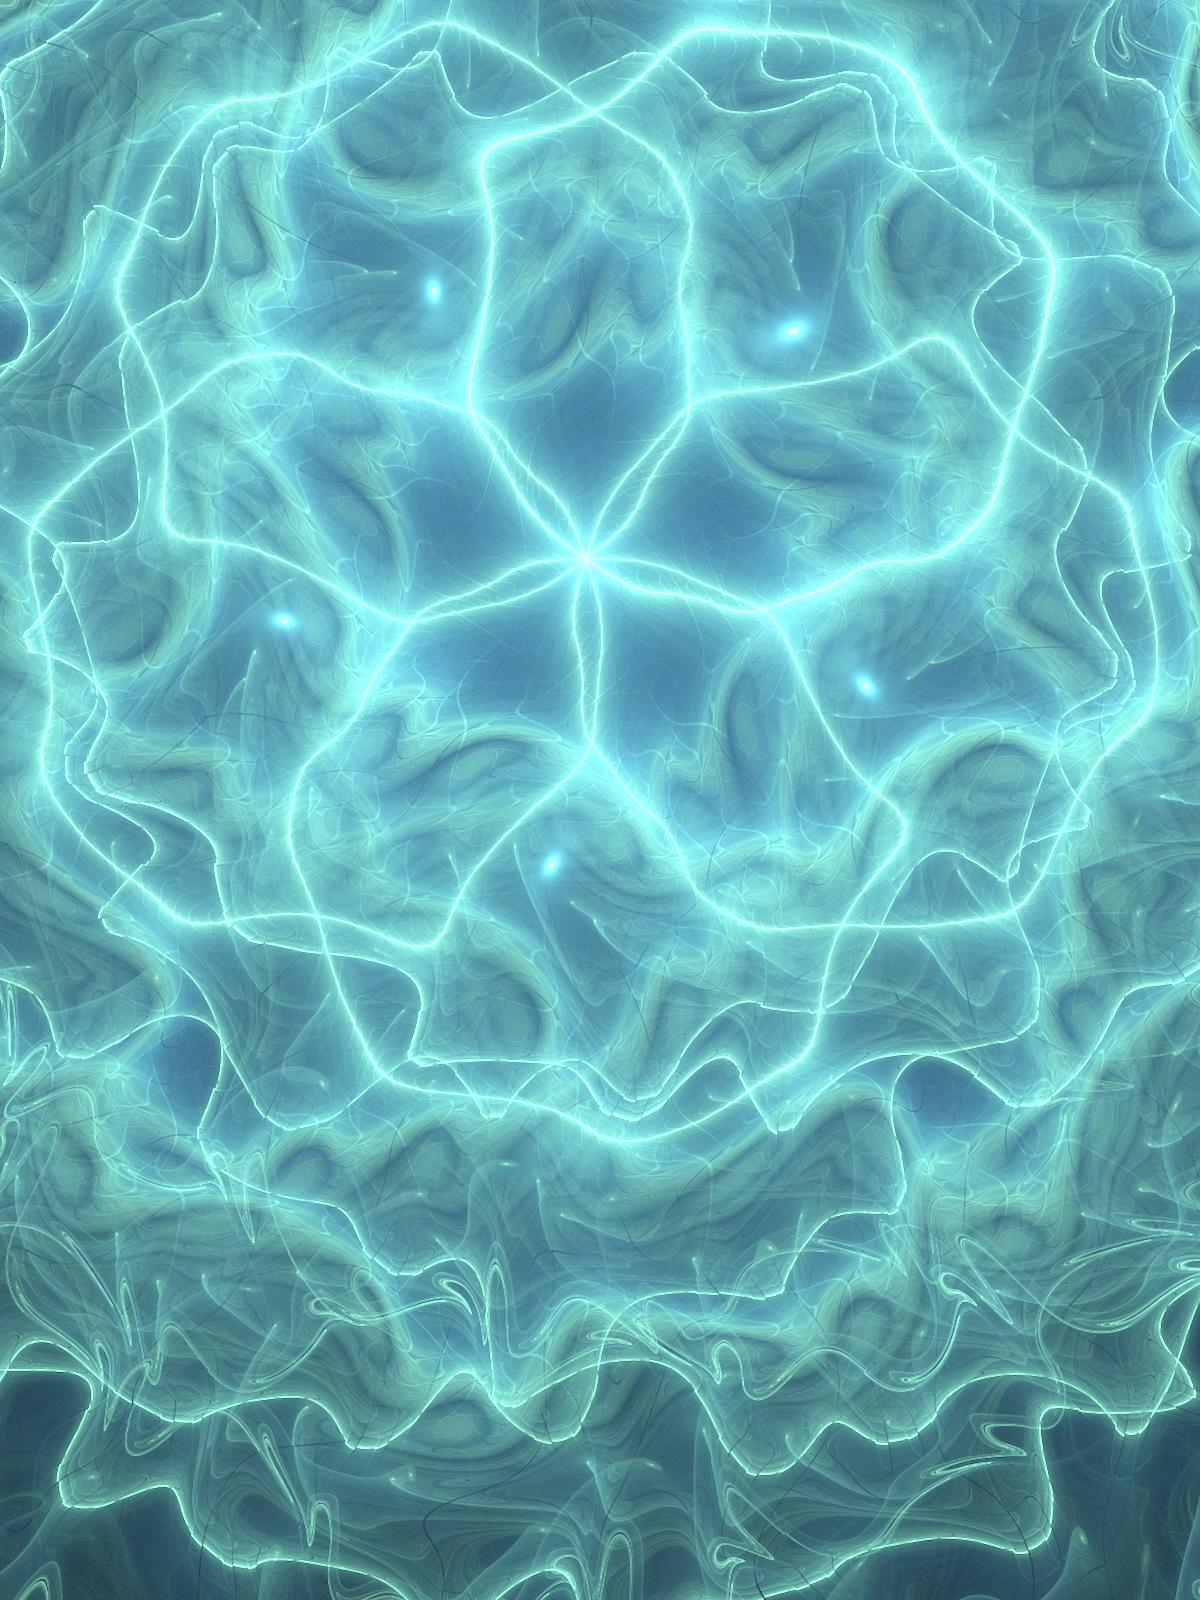
\includegraphics[width=\paperwidth, height=\paperheight]{images/blueback.jpg}};


    

      \begin{scope}[
        shift={(\pagewidth/2, -15cm)},
        draw=white,
        scale=1
      ]
        
        % Define the vector field function
        % Based on Van der Pol's equation with mu=0.08
        \def\vectorfieldx(#1,#2){0.08 * (1 - (#2)^2) * (#1) - (#2)}
        \def\vectorfieldy(#1,#2){(#1)}

        % Draw the vector field
        \foreach \x in {-10,-9.4,...,10}
            \foreach \y in {-6,-5.4,...,6}
            {
                % Calculate the vector at (\x, \y)
                \pgfmathsetmacro\vx{\vectorfieldx(\x,\y)}
                \pgfmathsetmacro\vy{\vectorfieldy(\x,\y)}
                
                % Normalize the vector for consistent arrow lengths
                \pgfmathsetmacro\norm{sqrt(\vx*\vx + \vy*\vy + 0.01)}
                \pgfmathsetmacro\scaleChange{atan(\norm)/100/\norm}
                \pgfmathsetmacro\vx{\vx*\scaleChange}
                \pgfmathsetmacro\vy{\vy*\scaleChange}
                            
                % Draw the vector as an arrow
                \draw[->] (\x,\y) -- ++(\vx,\vy);
            }

        
      \end{scope}



		\fill[path fading=north,covershade] (0,2.2in) rectangle ([yshift=-1.01in, xshift=2pt]current page.north east);
		\fill[covershade] (0,-1in) rectangle ([yshift=-2.05in]current page.north east);
		\fill[path fading=south, covershade] (0,-2in) rectangle ([xshift=1in,yshift=2in]current page.south east);
	\end{scope}


      \begin{scope}[
        shift={(\pagewidth/2, -15cm)},
        draw=white,
        scale=1
      ]
      \draw[very thick, coverblue] plot[smooth] coordinates {
        (-12.0, 7.0)
        (-7.767707632117724, 5.1136037435947825)
        (-6.55029161639424, 3.7063587117266086)
        (-6.291033918196791, 2.431866228538724)
        (-6.411138793864125, 1.1650517227439243)
        (-6.576468000195089, -0.1356950131526572)
        (-6.44221813555265, -1.4455579004483055)
        (-5.698360207820413, -2.6712777707594126)
        (-4.3170951341152985, -3.681408536248483)
        (-2.6524880454540365, -4.37905302197615)
        (-1.1398165469806572, -4.75315228434578)
        (0.01328155024075596, -4.859475753823552)
        (0.821915312513845, -4.770966774085827)
        (1.3846383135974278, -4.547077407312887)
        (1.7961623140784613, -4.227124320660122)
        (2.123678809225348, -3.8341569115250524)
        (2.4094036113245103, -3.3803996968979177)
        (2.6775274852229343, -2.8715397422619997)
        (2.9386885084803342, -2.3098255535481886)
        (3.190838170593432, -1.69663243845697)
        (3.4170363882183348, -1.0351789558166329)
        (3.582009820736538, -0.33385542452399053)
        (3.6319003441010573, 0.38997593972207234)
        (3.5045429976954092, 1.1070520961664807)
        (3.155148685264799, 1.7768762090366046)
        (2.587887900921836, 2.354441418187956)
        (1.8672212901679928, 2.801721875585408)
        (1.092152607672107, 3.0977299491587664)
        (0.3521124991605785, 3.241010555474463)
        (-0.3012250732092604, 3.2444440764401086)
        (-0.8544424867297288, 3.1272473241910546)
        (-1.3177350297141097, 2.9086793500487116)
        (-1.709817254884819, 2.604896520292268)
        (-2.0481012160157013, 2.2283238912763963)
        (-2.3434557798857867, 1.7884967847522988)
        (-2.5972850709562825, 1.2936842300215976)
        (-2.7995318396515483, 0.7529934864707473)
        (-2.9278428747642637, 0.17877669679455344)
        (-2.9498722041815304, -0.4110641575659039)
        (-2.8314891836259553, -0.991783374275332)
        (-2.5513563553185032, -1.532811519414777)
        (-2.1160520694453173, -2.0019036384168625)
        (-1.5647422912668723, -2.3714499982710877)
        (-0.9571888715832826, -2.624054645877739)
        (-0.35223637076719383, -2.7545420554150293)
        (0.208969609093618, -2.767917451822092)
        (0.7074017997129245, -2.6751774466319342)
        (1.1409678733905675, -2.4892999186199094)
        (1.5162256407417851, -2.2226802066727953)
        (1.8412312541603981, -1.8861516827108782)
        (2.1205905684074478, -1.4892157035815488)
        (2.352260492982905, -1.0410753957570995)
        (2.5256766930025374, -0.5521750545501195)
        (2.621620284466748, -0.03595560032841198)
        (2.6151475323385895, 0.489642956954491)
        (2.4828662364408713, 1.0016886486351866)
        (2.213661103089849, 1.4736108153020884)
        (1.8180343344692644, 1.87867104878967)
        (1.3293099813169997, 2.1945867570657827)
        (0.794190797901561, 2.4073061511888207)
        (0.25804987609744895, 2.51222531866222)
        (-0.24631674645531015, 2.512681356829908)
        (-0.7019367638291837, 2.416976971257817)
        (-1.1044256432520505, 2.2354636862561548)
        (-1.4562076752432407, 1.9785897841527467)
        (-1.7610609416378367, 1.6561027105679327)
        (-2.020002614298509, 1.277213574259159)
        (-2.228526532533583, 0.8514469679845532)
        (-2.375195446537731, 0.3899115410835035)
        (-2.4421349478709335, -0.09332365807743277)
        (-2.4084334761470485, -0.5802252701871604)
        (-2.256955233486863, -1.0488170439950872)
        (-1.9829845793569496, -1.4747978246149418)
        (-1.6003924258753368, -1.8347279568172121)
        (-1.1406761821858395, -2.109792485846884)
        (-0.6442804956115891, -2.2885599794563785)
        (-0.14905669061228027, -2.3676084893799945)
        (0.31787754049255496, -2.35009818117491)
        (0.7421113276838633, -2.2433266310881654)
        (1.119138965567409, -2.0564122105339555)
        (1.4496729869999478, -1.7987719532965614)
        (1.7351596765093849, -1.479539797410572)
        (1.9743152064050415, -1.1077853339754915)
        (2.1608397452464505, -0.6933087834541305)
        (2.2825158087168145, -0.2477611748453797)
        (2.3222938452721924, 0.2142407036486867)
        (2.2621209451040585, 0.6744809719789223)
        (2.0894657385199515, 1.1115611348709173)
        (1.8045089626601378, 1.5027415833371311)
        (1.4240855299322206, 1.8269671904607552)
        (0.9791376348682078, 2.06806108994217)
        (0.5063439362135758, 2.216775540958691)
        (0.03852092207133201, 2.2709535708439934)
        (-0.4014265867003714, 2.2340673110395572)
        (-0.8014088727874329, 2.1130654636693826)
        (-1.1573756131866144, 1.9164467311945423)
        (-1.4691961632545818, 1.6530581640768567)
        (-1.7367949045428668, 1.3317096385534777)
        (-1.9571899726047706, 0.961476199282158)
        (-2.1226527145621805, 0.5524838313440343)
        (-2.2203103862699436, 0.116926977800035)
        (-2.2338013602251845, -0.3300282070157654)
        (-2.1474985307327685, -0.7699250501521737)
        (-1.9527863128114766, -1.1817704006299714)
        (-1.6540334248527286, -1.5440681719746923)
        (-1.270731360880768, -1.837720725007975)
        (-0.8336872859941531, -2.0487709476862106)
        (-0.3768634432605625, -2.169889208925666)
        (0.07077143527120053, -2.200151187280596)
        (0.489693712624652, -2.143516599092316)
        (0.8698389827891272, -2.00687369097906)
        (1.2077367718350809, -1.7984036510000627)
        (1.502739299855169, -1.5266371015336484)
        (1.753602991749257, -1.2002432493885946)
        (1.9559428764769988, -0.8284203015062654)
        (2.1008147526865844, -0.421686841288038)
        (2.1748226436409226, 0.007186991769159341)
        (2.162328656981824, 0.4424707012207193)
        (2.0500252847240463, 0.8654457248214958)
        (1.8329280767882254, 1.2554641277632004)
        (1.51919861148228, 1.5921427727068889)
        (1.130697399744855, 1.8581381762698097)
        (0.6981551997160884, 2.041483871058576)
        (0.2532616593047968, 2.1365911862081575)
        (-0.17824373392450243, 2.1437023482517903)
        (-0.579701459542237, 2.067316017148458)
        (-0.9428033294882393, 1.914390887493251)
        (-1.2646214979968802, 1.6929509253499995)
        (-1.5440907544260531, 1.4113626474013903)
        (-1.778947488670822, 1.0782809921866066)
        (-1.9635539369440294, 0.7031235251737777)
        (-2.087896818752325, 0.29686806026276125)
        (-2.138207129951642, -0.12710255097312514)
        (-2.0997089249039522, -0.5524859428559366)
        (-1.9614753387919905, -0.9603155336591611)
        (-1.7220506686066896, -1.3302995021981292)
        (-1.3931134923157114, -1.6431396923995158)
        (-0.998585021637545, -1.8831569144828317)
        (-0.5689931640011031, -2.0402388269692353)
        (-0.13391225551434208, -2.110404276892739)
        (0.28379833982423563, -2.094982022582439)
        (0.6699835181429457, -1.9990034251459907)
        (1.0178468630950517, -1.8295530054695943)
        (1.324897085026137, -1.59458761616797)
        (1.5896448967126573, -1.3024102069389991)
        (1.8088545791135953, -0.9617572738068034)
        (1.9757183707830477, -0.582348425224214)
        (2.0792788944052543, -0.175682874320757)
        (2.1055730240775365, 0.24421200152425207)
        (2.040895821914876, 0.6604698581912402)
        (1.8768516354841762, 1.0539219298799434)
        (1.61548542293274, 1.4046923420456525)
        (1.2717444025090485, 1.694599509255421)
        (0.8712641888363498, 1.9095973507364619)
        (0.44414108668166763, 2.041335554647893)
        (0.017852270600155092, 2.087326642373181)
        (-0.38740254880218733, 2.049897877495028)
        (-0.7596902706986574, 1.934578001084655)
        (-1.0934959761230514, 1.748594590246179)
        (-1.3866259077743752, 1.4998916361508758)
        (-1.6371070224778699, 1.1967822580892171)
        (-1.840730763384624, 0.8481640531758838)
        (-1.9895752022801223, 0.46413286364143536)
        (-2.0718681911500787, 0.05676532753024312)
        (-2.0736665367191685, -0.3592450468258276)
        (-1.9825969322903052, -0.7664950664560172)
        (-1.7929881991203853, -1.145688727688495)
        (-1.510370575292366, -1.4774608039737998)
        (-1.152691840336067, -1.7448119142012528)
        (-0.7469146918320778, -1.9353256694087746)
        (-0.322421488196114, -2.0423399087455065)
        (0.09545032880050824, -2.0647536473458064)
        (0.4889962171687081, -2.005799354548482)
        (0.8482580152449181, -1.8714531921246096)
        (1.1687789621135087, -1.6690841403991947)
        (1.448507639830574, -1.4066598010739297)
    };
      \end{scope}



\newcommand{\titletext}[5]{
	\draw (#1, #2) node[right,opacity=0.55] {	
		\textpdfrender{
		    TextRenderingMode=Fill,
		    LineWidth=1pt,
		    FillColor=#4,
		  }{\fontsize{#5}{100}\fontfamily{phv}\selectfont  \bfseries #3}
	};
	\draw (#1, #2) node[right] {	
		\textpdfrender{
		    TextRenderingMode=Stroke,
		    LineWidth=1pt,
		    StrokeColor=#4,
		  }{\fontsize{#5}{100}\fontfamily{phv}\selectfont  \bfseries #3}
	};
}

\newcommand{\subtitletext}[5]{
	\draw (#1, #2) node[right,opacity=0.55] {	
		\textpdfrender{
		    TextRenderingMode=Fill,
		    LineWidth=1pt,
		    FillColor=#4,
		  }{\fontsize{#5}{100}\fontfamily{phv}\selectfont #3}
	};
	\draw (#1, #2) node[right] {	
		\textpdfrender{
		    TextRenderingMode=Stroke,
		    LineWidth=1pt,
		    StrokeColor=#4,
		  }{\fontsize{#5}{100}\fontfamily{phv}\selectfont #3}
	};
}




  \begin{scope}[yscale=-1, xscale=1, x=2.7pt, y=2.7pt,line join=miter,line cap=butt,line width=1.3pt, yshift=2.3cm, xshift=.7cm,
	  ]

	\coordinate (SUB) at (141, 30);

\begin{bookonly}
	\titletext{6}{23}{Calculus II}{coverblue}{58}	
\end{bookonly}

\begin{displayonly}
	\titletext{6}{23}{Calculus II}{coverblue}{50}	
\end{displayonly}


%    \begin{scope}[yscale=-9.7, xscale=9.7, yshift=-.96in]
%	  \fill[coverblue, opacity=.7] \LINEARALGEBRAoutline;
%	  \draw[coverblue, line width=1.3pt] \LINEARALGEBRAoutline;
%    \end{scope}
  \end{scope}
%


  

	\path[white] (SUB) node[anchor=north west] {\Large \bfseries \sffamily \coversubtitle};



\newcommand{\authornames}{\huge \sffamily \bfseries \begin{tabular}{r}Geoff McGregor\\Arman Pannu\\Jason Siefken\\\end{tabular}}
	\newcommand{\ypadd}{.5em}
	\newcommand{\xpadd}{1em}


\begin{bookonly}
	\draw (0, -24) node[right, xshift=10em] (AUTHOR) {\phantom{\authornames}};	
\end{bookonly}
\begin{displayonly}
	\draw (0, -8.5) node[right, xshift=10em] (AUTHOR) {\phantom{\authornames}};	
\end{displayonly}


	\path let \p1 = (AUTHOR.north) in coordinate (Ab1) at (0,\y1+\ypadd);
	\path let \p1 = (AUTHOR.north east) in coordinate (Ab2) at (\x1+\xpadd,\y1+\ypadd);
	\path let \p1 = (AUTHOR.south east) in coordinate (Ab3) at (\x1+\xpadd,\y1-\ypadd);
	\path let \p1 = (AUTHOR.south) in coordinate (Ab4) at (0,\y1-\ypadd);

	\path[fill=covershade, path fading=west, opacity=.8] (Ab1) -- (Ab2) -- (Ab3) -- (Ab4);
	\draw[covershade!80!black, line width=1.3pt] (Ab1) -- (Ab2) -- (Ab3) -- (Ab4);
\begin{bookonly}
	\draw (0, -24) node[right, xshift=10em, white] (AUTHOR) {\authornames};
\end{bookonly}
\begin{displayonly}
	\draw (0, -8.5) node[right, xshift=10em, white] (AUTHOR) {\authornames};
\end{displayonly}

\end{tikzpicture}
